
This section should give you a general idea of how the interface to Hermes2D works
and help you start experimenting with your own projects.
% If you should skip everything but one section, this is it.


%%%%%%%%%%%%%%%%%%%%%%%%%%%%%%%%%%%%%%%%%%%%%%%%%%%%%%%%%%%%%%%%%%%%%%%%%%%%%%%%%%%%%%%%%%%%%%%%%%%%

\subsection{Creating a Mesh}

Every finite element computation starts with partitioning of the problem domain
into simple elements. Here, we will be using triangles and quadrilaterals.
Normally this is done by specialized mesh generators, but in simple cases we
can type the mesh file by hand, as shown below. This will also allow us to explain
concepts such as boundary markers. Moreover, thanks to the adaptive capabilities
of Hermes2D, you may find that in many cases you no longer need a mesh generator
and very fine meshes to obtain accurate results. All you need to do is partition
the domain very coarsely into several large elements.

Suppose we want to define an L-shaped domain with a rounded corner, as shown in
Figure~\ref{fig:simplemesh}. The domain has already been partitioned into four large
elements, two quadrilaterals and two curvilinear triangles, each numbered from 0 to 3.
We also need to number all vertices of the mesh and assign markers to boundary edges.
These will be used later for creating boundary conditions.

\begin{figure}[ht]
  \smallskip\centering
  \includegraphics[width=0.52\textwidth]{img/simplemesh}
  \caption{Node and element numbering on an L-shaped domain.}
  \label{fig:simplemesh}
\end{figure}

Hermes2D uses a very simple mesh file format which we will use to describe the above
domain. You can find the complete mesh file here: {\tt hermes2d/ examples/01-mesh/domain.mesh}.
The file consists of variable assignments. Each variable can hold a real number,
a list of real numbers or a list of lists. The following are all valid definitions
in the Hermes2D mesh file format:
\index{Mesh!file format}

\lstset{language=make}
\begin{lstlisting}
# comments start with a hash
var = 5.0 + cos(pi)  # number
list = { 1, 2, 3, 4, var }  # list
pairs = { {1, 2}, {1, var}, {0, list} }  # list of lists
\end{lstlisting}

The mesh file must contain at least these variables: {\tt vertices}, {\tt elements} and
{\tt boundaries}. The variable {\tt vertices} must supply a list of coordinates of the
mesh vertices and in our case it may look like this:

\begin{lstlisting}
a = 1.0  # size of the mesh
b = sqrt(2)/2

vertices =
{
  { 0, -a },    # vertex 0
  { a, -a },    # vertex 1
  { -a, 0 },    # vertex 2
  { 0, 0 },     # vertex 3
  { a, 0 },     # vertex 4
  { -a, a },    # vertex 5
  { 0, a },     # vertex 6
  { a*b, a*b }  # vertex 7
}
\end{lstlisting}

The variable {\tt elements} lists all elements in the mesh.
Elements are defined by the (zero-based) indices of their vertices in
counter-clockwise order, and an extra number, denoting the element marker.
Element markers can be used to distinguish areas of the domain with different
material parameters, but normally all elements are assigned zero markers.
\index{Marker!element}

\begin{lstlisting}
elements =
{
  { 0, 1, 4, 3, 0 },  # quad 0
  { 3, 4, 7, 0 },     # tri 1
  { 3, 7, 6, 0 },     # tri 2
  { 2, 3, 6, 5, 0 }   # quad 3
}
\end{lstlisting}

\index{Marker!boundary}
The last mandatory variable, {\tt boundaries}, assigns boundary markers to
all boundary edges. By default, all edges have zero markers. Only those with
positive markers are considered lying on the domain boundary and can be
assigned a boundary condition, as we will see later.
An edge is identified by two vertex indices.

\begin{lstlisting}
boundaries =
{
  { 0, 1, 1 },
  { 1, 4, 2 },
  { 3, 0, 4 },
  { 4, 7, 2 },
  { 7, 6, 2 },
  { 2, 3, 4 },
  { 6, 5, 2 },
  { 5, 2, 3 }
}
\end{lstlisting}

Finally, the file can also include the variable {\tt curves}, which lists all curved edges.
Each curved edge is described by one NURBS curve, defined by its degree, control points and
knot vector. Simplified syntax is available for circular arcs.
More details on curved edges can be found in
Section~\ref{sec:nurbs}.
\index{NURBS}

\begin{lstlisting}
curves =
{
  { 4, 7, 45 },  # +45 degree circular arcs
  { 7, 6, 45 }
}
# EOF
\end{lstlisting}


%%%%%%%%%%%%%%%%%%%%%%%%%%%%%%%%%%%%%%%%%%%%%%%%%%%%%%%%%%%%%%%%%%%%%%%%%%%%%%%%%%%%%%%%%%%%%%%%%%%%

\subsection{Loading and Viewing a Mesh}

\index{Mesh!loading}
\index{Mesh!viewing}
Let us start with a ``Hello world'' example of using Hermes2D. We will load the mesh
we have just created and display it in a window.

\lstset{language=C++}
\begin{lstlisting}
#include "hermes2d.h"

int main(int argc, char* argv[])
{
  // load the mesh file
  Mesh mesh;
  mesh.load("domain.mesh");
  mesh.refine_element(1);
  mesh.refine_element(2);

  // display the mesh
  MeshView mview("Hello world!", 100, 100, 500, 500);
  mview.show(&mesh);

  // wait until the user closes the MeshView window
  View::wait();
  return 0;
}
\end{lstlisting}

First, an instance of the class {\tt Mesh} is created. If you are
a~C~programmer, you can think of a~class as a~{\tt struct} that also contains functions
(called methods in C++), that operate on the data members of the structure.
The class {\tt Mesh} contains the method {\tt load()}, which is used to load our mesh file.

Right after loading the mesh, we refined (subdivided) two of its elements. It does not
matter if the mesh becomes irregular, in fact, this is fully supported. You can also
refine all elements in the mesh by calling the method \verb"Mesh::refine_all_elements".
See Section~\ref{sec:meshmethods} for other ways of modifying meshes on the fly.

Finally, an object of the class {\tt MeshView} is created. You can initialize it by
supplying the title of the window and its initial position and size (all of these
parameters are optional). {\tt MeshView} provides the method {\tt show}, which
displays a window showing the mesh, see Figure~\ref{fig:meshview}.

At the end of the program, you may want to call the method {\tt View::wait()} to pause
the program, so that you have a chance to see its windows.

\begin{figure}[h!]
  \centering\medskip
  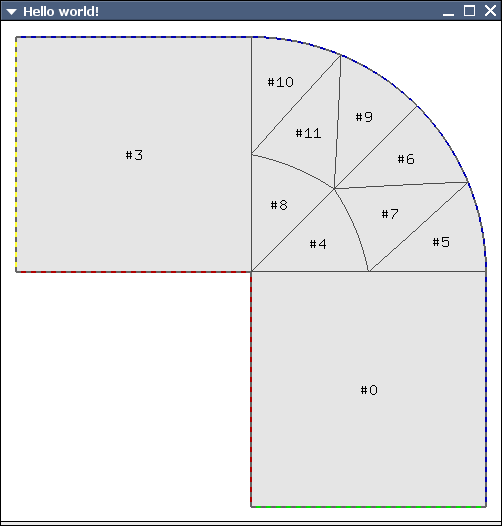
\includegraphics[width=0.52\textwidth]{img/meshview.png}
  \caption{MeshView visualization window.}
  \label{fig:meshview}
\end{figure}


%%%%%%%%%%%%%%%%%%%%%%%%%%%%%%%%%%%%%%%%%%%%%%%%%%%%%%%%%%%%%%%%%%%%%%%%%%%%%%%%%%%%%%%%%%%%%%%%%%%%

\subsection{Setting up a Finite Element Space}

\index{Space!creating}
With the mesh definition in place we can start preparing the finite element calculation.
Hermes2D follows closely the mathematical concept of finite element space in the
sense that you are required to construct a specific function space on top of a mesh
(ie., domain) before performing any FE calculation. Three predefined spaces are currently
available:
\begin{itemize}
  \item {\tt H1Space} -- \index{Space!$H^1$} the most common space of continuous,
        piecewise-polynomial functions belonging to $H^1(\Omega) = \{ v \in L^2(\Omega);
        \nabla u \in (L^2(\Omega))^2 \}$,
  \item {\tt HcurlSpace} -- \index{Space!$\Hcurl$} the space of vector-valued functions with
        continuous tangential components $\bfH(\mbox{curl},\Omega) = \{ \bfE \in (L^2(\Omega))^2;
        \nabla \times \bfE \in L^2(\Omega)\}$,
  \item {\tt L2Space} -- \index{Space!$L^2$} the space of functions discontinuous along mesh edges,
        belonging to the space $L^2(\Omega)$.
\end{itemize}

\index{Function!basis} \index{Function!edge} \index{Function!bubble}
All of these spaces allow higher-order elements and meshes with hanging nodes.
If you are not familiar with higher-order FEM, let us just say that in addition
to the standard linear pyramid-like vertex basis functions, the spaces can contain
quadratic, cubic, etc., {\em edge functions}, which generate higher-degree
polynomials along mesh edges, and {\em bubble functions}, which complete the higher-order
approximation in element interiors. The edge functions always span two neighboring
elements, while the support of bubble functions always coincides with
one element (see Figure \ref{fig:basisfn}).

\begin{figure}[ht]
  \centering\bigskip
  \includegraphics[width=\textwidth]{img/basisfn.jpg}
  \caption{\centering Fourth-order edge function (left) and \\
           one of the fifth-order bubble functions (right).}
  \label{fig:basisfn}
\end{figure}

There are many possible ways of constructing the polynomials which define the
higher-order basis functions. A particular set of polynomials is called
\emph{shapeset}\index{Shapeset}. Hermes2D defines several different shapesets from which
you need to choose when creating a FE space. The ones which perform best
(according to our experience) are simply called {\tt H1Shapeset} and {\tt HcurlShapeset}.
Others can be found in the files {\tt shapeset\_*\_all.h}. A single shapeset
can be used for more than one space.

We are now ready for an example. The following code snippets come from
\verb"hermes2d/examples/02-space/main.cpp". We assume that a mesh has already
been loaded. First we create an instance of {\tt H1Shapeset} and then an
instance of {\tt H1Space}, supplying the mesh and shapeset pointers:

\begin{lstlisting}
 // create a shapeset and an H1 space
 H1Shapeset shapeset;
 H1Space space(&mesh, &shapeset);
\end{lstlisting}

After the space has been created we need to initialize the polynomial
degrees\footnote{We use the terms \emph{degree} and \emph{order} interchangeably.}
of the elements. This can be done for individual elements by calling the method
\verb"Space::set_element_order()", or for all elements at once using
\verb"Space::set_uniform_order()". It is important to note that element degrees
are stored in the {\tt Space}, not in the {\tt Mesh}. The reason is that you can
have multiple different spaces with different element degrees over the same mesh.
In Hermes2D the mesh only stores geometrical information.

\begin{lstlisting}
 // assign element orders
 space.set_uniform_order(5);
\end{lstlisting}

A space created in this way is ready for use. By default, it is equipped with
zero Dirichlet boundary condition on the entire domain boundary. We will see
how to change that in Section \ref{sec:bc}.

\index{Space!viewing}
As a debugging feature, Hermes2D provides a visualization window for the
examination of the basis functions defined by a space. Similarly to {\tt MeshView},
you can create a {\tt BaseView} object and use it to display a space.
You can then cycle through all basis functions in the window using the arrow keys.

\begin{lstlisting}
 // view the basis functions
 BaseView bview;
 bview.show(&space);
\end{lstlisting}

This is how Figure \ref{fig:basisfn} was obtained (press the ``{\tt 3}'' key for 3D mode).
You can experiment with element refinements and hanging nodes to see how
irregular meshes are handled.

More details on the space classes can be found in Section \ref{sec:space}.


%%%%%%%%%%%%%%%%%%%%%%%%%%%%%%%%%%%%%%%%%%%%%%%%%%%%%%%%%%%%%%%%%%%%%%%%%%%%%%%%%%%%%%%%%%%%%%%%%%%%

\subsection{Solving the Poisson Equation}
\label{sec:poisson}
\index{Poisson equation}

Let us solve the Poisson equation on our L-shaped domain $\Omega$ with zero Dirichlet boundary
condition:
$$-\Delta u = 2,\ \ \ \ \ \ u = 0\,\ \mbox{on}\,\ \partial \Omega.$$
The weak formulation \index{Weak formulation} for this equation reads
\begin{equation} \label{poissonweak}
  \int_\Omega \nabla u \cdot \nabla v \;\mbox{d\bfx} = 2 \int_\Omega v \;\mbox{d\bfx}
\end{equation}
where $u$, $v$ belong to the $H^1$ space we defined in the previous section.
Equation (\ref{poissonweak}) has the standard form $a(u,v) = l(v)$ and we need
a way to specify the bilinear form $a(u,v)$ and the linear form $l(v)$.
\index{Bilinear form} \index{Linear form}
In the code this is done by implementing the following two functions:

\begin{lstlisting}
scalar bilinear_form(RealFunction* fu, RealFunction* fv,
                     RefMap* ru, RefMap* rv);

scalar linear_form(RealFunction* fv, RefMap* rv);
\end{lstlisting}

These functions will be called for each element during the stiffness matrix
assembly and must return the values of the bilinear and linear forms for the given arguments.
{\tt RealFunction} represents one of the basis functions restricted to the
current element and {\tt RefMap} represents the reference mapping of the current element.
There are methods for extracting the values of the basis functions at integration points,
which allows you to evaluate the integrals by yourself, but this is normally not needed,
since many common weak forms have already been implemented: see Appendix
\ref{ch:integralforms}. In this case, we can simply use the predefined functions
\verb"int_grad_u_grad_v" and \verb"int_v":

\begin{lstlisting}
scalar bilinear_form(RealFunction* fu, RealFunction* fv,
                     RefMap* ru, RefMap* rv)
{
  return int_grad_u_grad_v(fu, fv, ru, rv);
}

scalar linear_form(RealFunction* fv, RefMap* rv)
{
  return 2*int_v(fv, rv);
}
\end{lstlisting}


We can now state our problem in the following way
(taken from {\tt hermes2d/ examples/03-poisson}):

\begin{lstlisting}
 // initialize the weak formulation
 WeakForm wf(1); // num. eq.
 wf.add_biform(0, 0, bilinear_form);
 wf.add_liform(0, linear_form);
\end{lstlisting}
\index{WeakForm}

The class {\tt WeakForm} represents the weak formulation of the PDE and must be
initialized with the number of equations in the system, in our case one. We then
gave the class pointers to our bilinear and linear form functions.
The numbers in {\tt add\_biform} and {\tt add\_liform} will be explained in
Section \ref{sec:systems}.

Given the weak formulation and the discretization determined by the space and its mesh,
we can proceed to the approximate solution of the problem by the Galerkin method.
This method is the core of Hermes2D and provides a way to obtain a sparse linear
system of equations, represented by the class {\tt LinSystem} in the code. The solution
of the linear system then yields an approximate solution of the original problem.
\index{LinSystem}
\index{Galerkin method}

The class {\tt LinSystem} needs three things: your weak formulation, your spaces and
finally an external sparse linear solver, for example UMFPACK. The following lines
create the linear solver, initialize the {\tt LinSystem} class and pass a pointer to
the {\tt H1Space} we have created in the previous section.

\begin{lstlisting}
 // initialize the linear system and solver
 UmfpackSolver umfpack;
 LinSystem sys(&wf, &umfpack);
 sys.set_spaces(1, &space);
 sys.set_pss(1, &pss);
\end{lstlisting}

The last line must be included for historical reasons. During matrix assembly,
Hermes2D caches the values of all shape function polynomials for better performance.
The cache is represented by the class {\tt PrecalcShapeset} and you have to
include the following line at the beginning your program:

\begin{lstlisting}
 PrecalcShapeset pss(&shapeset);
\end{lstlisting}

Finally, we tell {\tt LinSystem} to assemble the stiffness matrix and the right-hand
side and solve the resulting linear system: \index{Stiffness matrix}

\begin{lstlisting}
 // assemble the stiffness matrix and solve the system
 Solution sln;
 sys.assemble();
 sys.solve(1, &sln);
\end{lstlisting}

The last two lines can be repeated many times in time-dependent problems. Here,
however, we are finished. The instance of the class {\tt Solution}, upon the
completion of {\tt LinSystem::solve}, contains the approximate solution of
the PDE. You can ask for its values, as described in Section \ref{sec:solution},
or you can visualize the solution immediately using the {\tt ScalarView} class:
\index{ScalarView}

\begin{lstlisting}
 // visualize the solution
 ScalarView view("Solution");
 view.show(&sln);
\end{lstlisting}

Figure \ref{fig:poissoncomplete} lists the complete source code for this example.
Figure \ref{fig:poisson} shows its output.

\begin{figure}[ht]
  \centering\medskip
  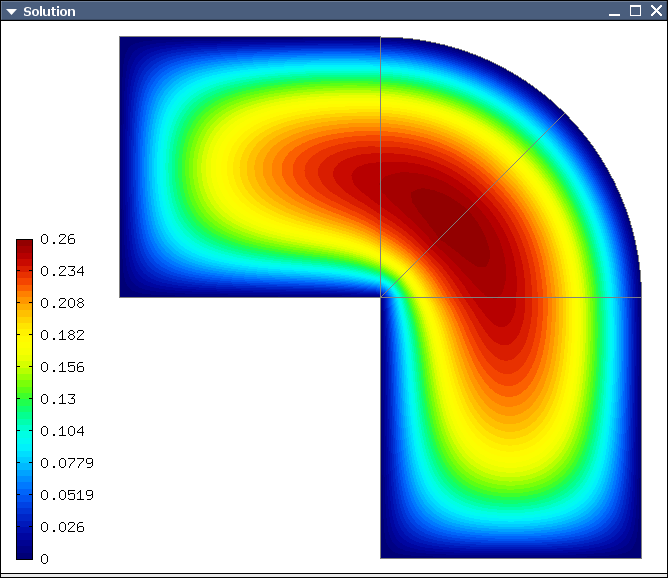
\includegraphics[width=0.75\textwidth]{img/poisson.png}
  \caption{Solution of the Poisson equation.}
  \label{fig:poisson}
\end{figure}



\begin{figure}[p]
  %\lstinputlisting{../examples/03-poisson/main.cpp}
\begin{lstlisting}
#include "hermes2d.h"
#include "solver_umfpack.h"  // defines the class UmfpackSolver

scalar bilinear_form(RealFunction* fu, RealFunction* fv,
                     RefMap* ru, RefMap* rv)
{
  return int_grad_u_grad_v(fu, fv, ru, rv);
}

scalar linear_form(RealFunction* fv, RefMap* rv)
{
  return 2*int_v(fv, rv);
}

int main(int argc, char* argv[])
{
  Mesh mesh;
  mesh.load("domain.mesh");
  mesh.refine_element(0);

  // initialize the shapeset and the cache
  H1Shapeset shapeset;
  PrecalcShapeset pss(&shapeset);

  // create an H1 space
  H1Space space(&mesh, &shapeset);
  space.set_uniform_order(5);
  space.assign_dofs();

  // initialize the weak formulation
  WeakForm wf(1);
  wf.add_biform(0, 0, bilinear_form);
  wf.add_liform(0, linear_form);

  // initialize the linear system and solver
  UmfpackSolver umfpack;
  LinSystem sys(&wf, &umfpack);
  sys.set_spaces(1, &space);
  sys.set_pss(1, &pss);

  // assemble the stiffness matrix and solve the system
  Solution sln;
  sys.assemble();
  sys.solve(1, &sln);

  // visualize the solution
  ScalarView view("Solution");
  view.show(&sln);
  View::wait();
  return 0;
}
\end{lstlisting}
  \vspace{-2mm}
  \caption{Complete listing of the Poisson equation example.}
  \label{fig:poissoncomplete}
\end{figure}


%%%%%%%%%%%%%%%%%%%%%%%%%%%%%%%%%%%%%%%%%%%%%%%%%%%%%%%%%%%%%%%%%%%%%%%%%%%%%%%%%%%%%%%%%%%%%%%%%%%%

\subsection{Adding Boundary Conditions}
\label{sec:bc}

\index{Boundary conditions!essential vs. natural}
Hermes2D recognizes two kinds of boundary conditions: {\em essential} and {\em natural}.
Essential boundary conditions influence and modify the finite element space while natural
conditions do not (they are incorporated into boundary integrals in the weak formulation).
In the context of elliptic problems, Dirichlet conditions are essential and Neumann/Newton
conditions are natural.

% -----------------------------------------------------------------------------------------

\subsubsection{Dirichlet Boundary Condition}

\index{Boundary conditions!Dirichlet}
Since essential conditions remove degrees of freedom (DOFs) from the FE space, they need to be
specified when setting the space up. This is done by providing the following two callback functions:

\begin{lstlisting}
int bc_types(int marker);
scalar bc_values(int marker, double x, double y);
\end{lstlisting}

The first one, given the boundary marker number, determines the type of BC which the associated
portion of the domain boundary belongs to, by returning one of the predefined constants \verb"BC_ESSENTIAL"
or \verb"BC_NATURAL". The second callback returns the value of the BC for a given marker and
position on the boundary (see Section \ref{sec:space} for more details and alternatives). The space
initialization might then look as follows:

\begin{lstlisting}
 H1Space space(&mesh, &shapeset);
 space.set_bc_types(bc_types);
 space.set_bc_values(bc_values);
\end{lstlisting}

Suppose we would like to modify our model problem in the following way:
$$-\Delta u = -4,\ \ \ \ \ \ u = x^2 + y^2\,\ \mbox{on}\,\ \partial \Omega.$$
Besides changing the linear form, we need to specify that all the boundary markers 1, 2, 3, 4
(refer to Figure \ref{fig:simplemesh} on page \pageref{fig:simplemesh}) denote the essential
boundary condition:

\begin{lstlisting}
int bc_types(int marker)
{
  return BC_ESSENTIAL;
}
\end{lstlisting}

Further, the value callback must return the value of our Dirichlet BC:

\begin{lstlisting}
scalar bc_values(int marker, double x, double y)
{
  return x*x + y*y;
}
\end{lstlisting}

It is clear that the solution to this problem is the function $u = x^2 + y^2$, as shown
in Figure \ref{fig:dirichlet}, which is the output of the example
{\tt 04-bc-dirichlet}.

\begin{figure}[ht]
  \centering\medskip
  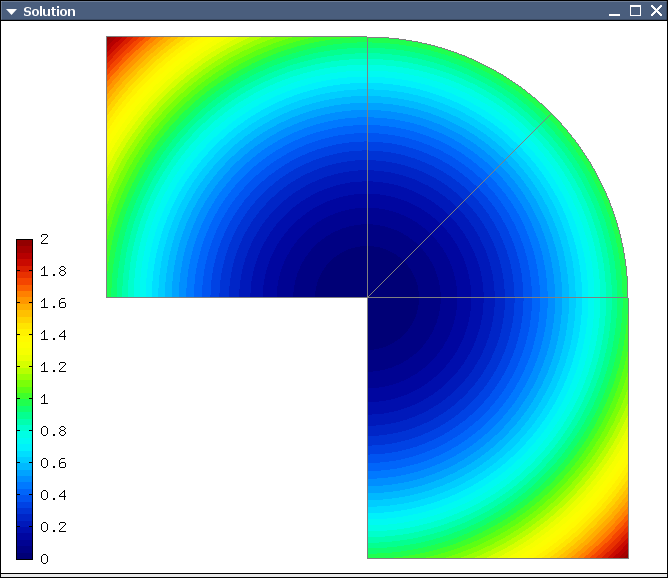
\includegraphics[width=0.7\textwidth]{img/dirichlet.png}
  \caption{Solution of the Dirichlet problem.}
  \label{fig:dirichlet}
\end{figure}

% -----------------------------------------------------------------------------------------

\subsubsection{Neumann Boundary Condition}

\index{Boundary conditions!Neumann}
Next, let us add the Neumann BC. The new problem will be
\begin{eqnarray*}
  -\Delta u = -1,\ \ \ \ \ &&u = 0\,\ \mbox{on}\,\ \Gamma_4,\\
                           &&\dd{u}{n} = 0\,\ \mbox{on}\,\ \Gamma_1 \cup \Gamma_3,\\
                           &&\dd{u}{n} = 1\,\ \mbox{on}\,\ \Gamma_2,
\end{eqnarray*}
where $\Gamma_1 \dots \Gamma_4$ correspond to the edges marked $1 \dots 4$ in Figure
\ref{fig:simplemesh}. Now, a~surface integral appears in the weak formulation:
$$\int_\Omega \nabla u \cdot \nabla v \;\mbox{d\bfx} =
  -\int_\Omega v \;\mbox{d\bfx} + \int_{\Gamma_2} \!v \;\mbox{d}l$$

In Hermes2D, all forms in the standard weak formulation $a(u,v) = l(v)$
are in fact defined as a sum of contributions from volume integrals and from
surface integrals. In the case of the linear form $l(v)$, this means
$$l(v) = \sum_m l_m^{\,\rm vol}(v) + \sum_n l_n^{\,\rm surf}(v).$$
We have already seen volume linear forms in Section \ref{sec:poisson}.
Surface linear forms are implemented similarly. Our new right-hand side will
be represented by two functions with the following prototypes:

\begin{lstlisting}
scalar linear_form     (RealFunction* fv, RefMap* rv);
scalar linear_form_surf(RealFunction* fv, RefMap* rv,
                        EdgePos* ep);
\end{lstlisting}

and will be added to the {\tt WeakForm} by the following code:

\begin{lstlisting}
  wf.add_liform(0, linear_form);
  wf.add_liform_surf(0, linear_form_surf_Gamma_2, 2);
\end{lstlisting}

Note that the optional third argument to both {\tt add\_liform} and {\tt add\_liform\_ surf}
restricts the evaluation of the form to a given element or boundary marker. In our
case, we only want the surface part of the linear form to be evaluated on $\Gamma_2$.
For better readability, this is also reflected in the name of the form. The surface
form itself contains the command

\begin{lstlisting}
 return 1.0 * surf_int_v(fv, rv, ep);
\end{lstlisting}

Here, we have used the predefined surface integral \verb"surf_int_v" (see Section
\ref{sec:surfint}). If the boundary condition was more complicated, we could also
have used \verb"surf_int_F_v", where {\tt F} stands for an arbitrary user-supplied
function returning the value $\partial u/\partial n$.

Passing marker number as the third argument to {\tt add\_liform} and others is
in fact a shortcut. In case the integration region is more complicated, such as
$\Gamma_N = \Gamma_2 \cup \Gamma_4$, you need to define an area
(see {\tt WeakForm::def\_area} in Section \ref{sec:weakform}) and pass its number.
The constant {\tt ANY} causes the form to be integrated over the whole domain
or its boundary and is the default value.

Refer to example {\tt 05-bc-neumann} for the complete code. The approximate solution
of the Nemann problem is shown in Figure \ref{fig:neumann}.

\begin{figure}[ht]
  \centering\medskip
  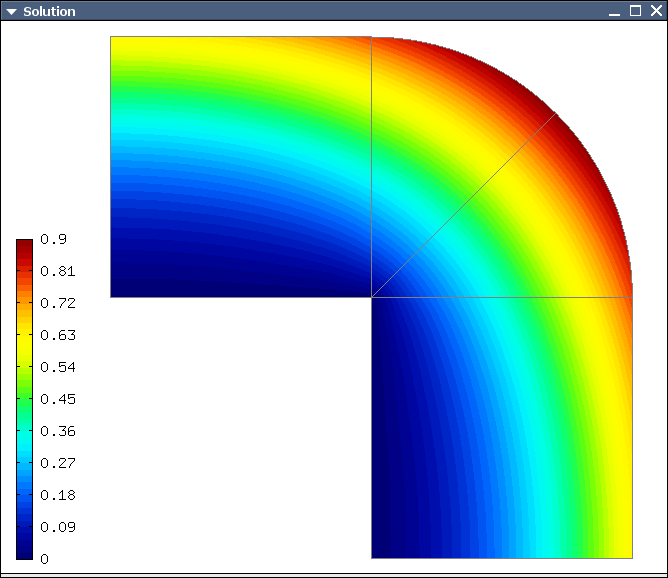
\includegraphics[width=0.7\textwidth]{img/neumann.png}
  \caption{Solution of the Neumann problem.}
  \label{fig:neumann}
\end{figure}

% -----------------------------------------------------------------------------------------

\subsubsection{Newton Boundary Condition}

\index{Boundary conditions!Newton}
\index{Boundary conditions!Robin}
Another common natural boundary condition is the Newton (sometimes called Robin) condition
of the form
$$\dd{u}{n} + c_1 u = c_2, \ \ \ \ c_1 \ne 0.$$
Like with the Neumann condition, this results in a surface integral appearing in the linear form,
but this time also in the bilinear form. Similarly to the linear form, the bilinear form is
a sum of volume and surface forms, that can be added to the weak formulation using the methods
{\tt add\_biform} and {\tt add\_biform\_surf} (see Section \ref{sec:weakform}).
The surface bilinear form must have the following prototype:

\begin{lstlisting}
scalar bilinear_form_surf(RealFunction* fu, RealFunction* fv,
                          RefMap* ru, RefMap* rv, EdgePos* ep);
\end{lstlisting}

Inside this function you can use forms such as \verb"surf_int_u_v", \verb"surf_int_F_u_v"; see
Section \ref{sec:surfint}. Example {\tt 06-bc-newton} demonstrates typical usage of the Newton
boundary condition on a stationary heat transfer problem, where one part of the boundary
represents a heat exchange surface obeying the Newton law of cooling.



%%%%%%%%%%%%%%%%%%%%%%%%%%%%%%%%%%%%%%%%%%%%%%%%%%%%%%%%%%%%%%%%%%%%%%%%%%%%%%%%%%%%%%%%%%%%%%%%%%%%

\subsection{Systems of PDEs}
\label{sec:systems}

\index{Weak formulation}
\index{System of PDEs}

So far we have seen the solution of a single linear PDE with the weak formulation
of the form $a(u,v) = l(v)$, where $u, v$ belong to one of the three predefined
function spaces. However, Hermes2D supports the solution of a system of $n$ linear
PDEs, provided its weak formulation can be written as follows:
\begin{eqnarray}
  a_{11}(u_1,v_1)\,+ a_{12}(u_2,v_1)\,+ \cdots\,+ a_{1n}(u_n,v_1) &=& l_1(v_1) \nonumber \\
  a_{21}(u_1,v_2)\,+ a_{22}(u_2,v_2)\,+ \cdots\,+ a_{2n}(u_n,v_2) &=& l_2(v_2) \label{weaksystem} \\
                                                      &\vdots&     \nonumber  \\
  a_{n1}(u_1,v_n) + a_{n2}(u_2,v_n) + \cdots + a_{nn}(u_n,v_n) &=& l_n(v_n). \nonumber
\end{eqnarray}
The solution $\bfu = (u_1, u_2, \dots, u_n)$ and test functions $\bfv =
(v_1, v_2, \dots, v_n)$ belong to the space $W = V_1 \times V_2 \times \dots
\times V_n$, where each $V_i$ is one of the available function spaces.

Let us illustrate this by solving a problem of linear elasticity. Consider a
two-dimensional axisymmetric elastic body shown in Figure \ref{elastsample}.
In the plane-strain model of linear elasticity the goal is to determine the
deformation of the body subject to the forces $f$. The deformation is sought
as a vector function $u(x) = (u_1, u_2)^T$, describing the displacement of each point
$x \in \Omega$ after the load $f = (f_1, f_2)^T$ is applied.

\begin{figure}[h]
  \vspace{-2mm}
  \medskip\centering
  \includegraphics[width=0.87\textwidth]{img/elastsample}
  \caption{Axisymmetric elastic body loaded on two sides.}
  \label{elastsample}
\end{figure}

The boundary conditions are
\begin{eqnarray}
  \dd{u_1}{n} \!&=&\! \left\{ \begin{array}{cl}
                                f_1 & \mbox{on} \ \Gamma_3 \\
                                0   & \mbox{elsewhere},
                              \end{array} \right \label{elastbc1}
  \\
  \dd{u_2}{n} \!&=&\! \left\{ \begin{array}{cl}
                                f_2 & \mbox{on} \ \Gamma_3 \\
                                0   & \mbox{on} \ \Gamma_2, \Gamma_4, \Gamma_5,
                              \end{array} \right \label{elastbc2}
  \\[2mm]
  u_2 \!&=&\! 0 \ \ \mbox{on} \ \Gamma_1. \label{elastbc3}
\end{eqnarray}

Applying the standard procedure to the elastostatic equilibrium equations
(see \cite{lifshitz}), we arrive at the following weak formulation:
\begin{eqnarray*}
  \int_\Omega
    (2\mu\!+\!\lambda)\dd{u_1}{x_1}\dd{v_1}{x_1} + \mu\dd{u_1}{x_2}\dd{v_1}{x_2} +
    \mu\dd{u_2}{x_1}\dd{v_1}{x_2} + \lambda\dd{u_2}{x_2}\dd{v_1}{x_1}
    \,\mbox{d}\bfx \!\!&=&\!\!\!
    %\int_\Omega \rho f_1 v_1 \,\mbox{d}\bfx +
    \int_{\Gamma_3} \!\!f_1 v_1 \,\mbox{d}S, \\ \smallskip
  \int_\Omega
    \mu\dd{u_1}{x_2}\dd{v_2}{x_1} + \lambda\dd{u_1}{x_1}\dd{v_2}{x_2} +
    (2\mu\!+\!\lambda)\dd{u_2}{x_2}\dd{v_2}{x_2} + \mu\dd{u_2}{x_1}\dd{v_2}{x_1}
    \,\mbox{d}\bfx \!\!&=&\!\!\!
    %\int_\Omega \rho f_2 v_2 \,\mbox{d}\bfx +
    \int_{\Gamma_3} \!\!f_2 v_2 \,\mbox{d}S.
\end{eqnarray*}

We see that the weak formulation can indeed be written in the form (\ref{weaksystem}):
\begin{eqnarray}
  a_{11}(u_1, v_1) \!&=&\! \int_\Omega (2\mu+\lambda)\dd{u_1}{x_1}\dd{v_1}{x_1} + \mu\dd{u_1}{x_2}\dd{v_1}{x_2} \,\mbox{d}\bfx, \label{sysform1} \\
  a_{12}(u_2, v_1) \!&=&\! \int_\Omega \mu\dd{u_2}{x_1}\dd{v_1}{x_2} + \lambda\dd{u_2}{x_2}\dd{v_1}{x_1} \,\mbox{d}\bfx,\\
  a_{21}(u_1, v_2) \!&=&\! \int_\Omega \mu\dd{u_1}{x_2}\dd{v_2}{x_1} + \lambda\dd{u_1}{x_1}\dd{v_2}{x_2} \,\mbox{d}\bfx,\\
  a_{22}(u_2, v_2) \!&=&\! \int_\Omega (2\mu+\lambda)\dd{u_2}{x_2}\dd{v_2}{x_2} + \mu\dd{u_2}{x_1}\dd{v_2}{x_1} \,\mbox{d}\bfx, \label{sysform2} \\
  l_{1}(v_1) \!&=&\!
  %\int_\Omega \rho f_1 v_1 \,\mbox{d}\bfx +
  \int_{\Gamma_3} \!\!f_1 v_1 \,\mbox{d}S, \\
  l_{2}(v_2) \!&=&\!
  %\int_\Omega \rho f_2 v_2 \,\mbox{d}\bfx +
  \int_{\Gamma_3} \!\!f_2 v_2 \,\mbox{d}S.  \label{sysform3}
\end{eqnarray}

Here, $\mu$ and $\lambda$ are material constants (Lam\'e coefficients) defined as
$$\mu = \frac{E}{2(1+\nu)}, \ \ \ \ \  \lambda = \frac{E\nu}{(1+\nu)(1-2\nu)},$$
where $E$ is the Young modulus and $\nu$ the Poisson ratio of the material. For
steel, we have $E = 200$ GPa and $\nu = 0.3$. The load is $f = (0, 10^4)^T$ N.

The mesh for the problem, as well as the code which we will refer to below,
can be found in \verb"examples/07-system".

We will again start by defining the function spaces for the two solution
components, $u_1$ and $u_2$ (the $x$ and $y$ displacement). The boundary
conditions (\ref{elastbc1})--(\ref{elastbc3}) can be implemented as
\begin{lstlisting}
 int bc_types_x(int marker)
   { return BC_NATURAL; }

 int bc_types_y(int marker)
   { return (marker == 1) ? BC_ESSENTIAL : BC_NATURAL; }

 double bc_values_y(EdgePos* ep)
   { return (ep->marker == 3) ? f : 0.0; }
\end{lstlisting}
We have omitted the callback {\tt bc\_values\_x} since it is zero (this is
the default BC value for any space). Next we create the two displacement spaces,
{\tt xdisp} and {\tt ydisp}:
\begin{lstlisting}
 // create the x displacement space
 H1Space xdisp(&mesh, &shapeset);
 xdisp.set_bc_types(bc_types_x);
 xdisp.set_uniform_order(8);

 // create the y displacement space
 H1Space ydisp(&mesh, &shapeset);
 ydisp.set_bc_types(bc_types_y);
 ydisp.set_bc_values(bc_values_y);
 ydisp.set_uniform_order(8);
\end{lstlisting}

Our {\tt WeakForm} instance will be initialized for two equations in the system.
After implementing the forms (\ref{sysform1})--(\ref{sysform2}) using the predefined integrals
{\tt int\_a\_dudx\_ dvdx\_b\_dudy\_dvdy} and {\tt int\_a\_dudx\_dvdy\_b\_dudy\_dvdx},
we can add them to the weak formulation using {\tt add\_biform}.
The first two parameters of this method correspond to the position of the form
in (\ref{weaksystem}) with zero-based numbering. Similarly for the surface linear form
(\ref{sysform3}).

\begin{lstlisting}
 // initialize the weak formulation
 WeakForm wf(2);
 wf.add_biform(0, 0, bilinear_form_0_0, SYM);
 wf.add_biform(0, 1, bilinear_form_0_1, SYM);
 wf.add_biform(1, 1, bilinear_form_1_1, SYM);
 wf.add_liform_surf(1, linear_form_1_surf);
\end{lstlisting}

An explanation of the extra parameter {\tt SYM} in {\tt add\_biform} is due.
Since the two diagonal forms $a_{11}$ and $a_{22}$ are symmetric, i.e.,
$a_{ii}(u,v) = a_{ii}(v,u)$, Hermes2D can be told to only evaluate them once for the
two cases $a_{ii}(u,v)$ and $a_{ii}(v,u)$ to speed up assembly. In fact, we should have
used the {\tt SYM} flag already in the previous sections, since the form
$a(u,v) = \nabla u \cdot \nabla v$ is also symmetric. This is however not the case
for all forms and the default value of the fourth parameter of {\tt add\_biform} is {\tt UNSYM}.

The off-diagonal forms $a_{12}(u_2, v_1)$ and $a_{21}(u_1, v_2)$ are not
(and cannot) be symmetric, since their arguments come from different spaces.
However, we can see that $a_{12}(u, v) = a_{21}(v, u)$, i.e., the corresponding blocks
of the local stiffness matrix are transposes of each other. Here, the {\tt SYM} flag
has a different effect: it tells Hermes2D to take the block of the local stiffness
matrix corresponding to the form $a_{12}$, transpose it and copy it where a block
corresponding to $a_{21}$ would belong, without evaluating $a_{21}$ at all (this is why
we don't add {\tt bilinear\_form\_1\_0}). This again speeds up the matrix assembly.
You can also use the flag {\tt ANTISYM}, which moreover inverts the sign of the block.
This makes sense in the case where $a_{ij}(u, v) = -a_{ji}(v, u)$.

It is recommended that you start with the default (and safe) {\tt UNSYM} flag for all
forms when developing your project, and only optimize the evaluation of the forms when
the code works well.

With the {\tt WeakForm} and spaces ready, we can initialize the linear system.
The only difference is that we now have two spaces determining the discretization
of the problem.

\begin{lstlisting}
 LinSystem sys(&wf, &umfpack);
 sys.set_spaces(2, &xdisp, &ydisp);
\end{lstlisting}

All that is left is to assemble the stiffness matrix and solve the system.
Since we have two equations and two spaces, we receive two solutions, one for each
displacement component:
\begin{lstlisting}
 Solution xsln, ysln;
 sys.assemble();
 sys.solve(2, &xsln, &ysln);
\end{lstlisting}

\smallskip As in the previous sections, it is now possible to visualize the displacement
solutions, e.g.,
\begin{lstlisting}
 ScalarView view("y displacement [m]");
 view.show(&ysln);
\end{lstlisting}
Usually, however, it is necessary to postprocess the solution in order to obtain more
informative visualization. In elasticity problems, one is often interested in material
stress, which is obtained by a formula combining the derivatives of the two displacements.
Hermes2D implements postprocessing through \emph{filters}. A filter is a special class
which takes up to three \verb"Solution"s, performs some computation and in the end acts
as another \verb"Solution", which can be visualized, or even fed into another filter.
Here, we can use the predefined filter \verb"VonMisesFilter", which calculates the
Von Mises stress:
\begin{lstlisting}
 VonMisesFilter stress(&xsln, &ysln, mu, lambda);
 view.show(&stress, EPS_HIGH, 0);
\end{lstlisting}
The second parameter of \verb"show" is the visualization accuracy and can be
\verb"EPS_LOW", \verb"EPS_NORMAL" (default) and \verb"EPS_HIGH". The third parameter is
the component number and is only valid for vector-valued (\Hcurl) solutions.

Finally, in elasticity problems, it may be illustrative to distort the computational
domain according to the calculated displacement. The function \verb"View::show" can be
passed three more optional parameters, which represent the $x$ and $y$ displacement
and a multiplier to make the displacements visible.
\begin{lstlisting}
 VonMisesFilter stress(&xsln, &ysln, mu, lambda);
 view.show(&stress, EPS_HIGH, 0, &xsln, &ysln, 1.5e5);
\end{lstlisting}

%The output of this code is shown in Figure \ref{elastsln}.

\begin{figure}[ht]
  \medskip \centering
  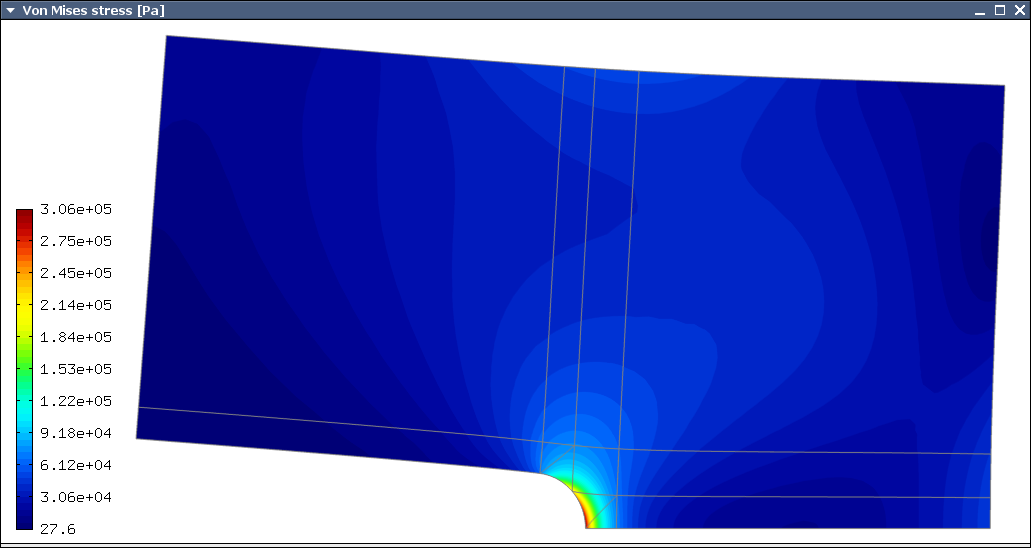
\includegraphics[width=\textwidth]{img/mises.png}
  \caption{Elastic stress plotted on deformed domain.}
  \label{elastsln}
\end{figure}


%%%%%%%%%%%%%%%%%%%%%%%%%%%%%%%%%%%%%%%%%%%%%%%%%%%%%%%%%%%%%%%%%%%%%%%%%%%%%%%%%%%%%%%%%%%%%%%%%%%%

\subsection{Time-dependent PDEs}

The approximate solution of many time-dependent and/or nonlinear problems is based on
an iterative scheme, in which it may be necessary to incorporate solutions from
previous iterations or time levels into the weak formulation of the problem.
This section describes the implementation of a simple transient Navier-Stokes solver
that can be found in {\tt examples/08-time-dep}.

\begin{figure}[b]
  \medskip \centering
  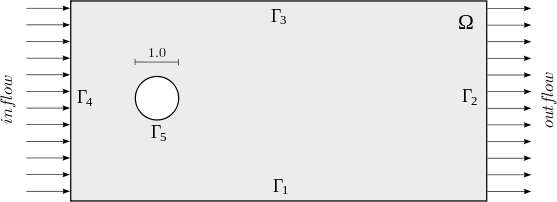
\includegraphics[width=0.95\textwidth]{img/cylinder}
  \caption{Domain for the Navier-Stokes problem.}
  \label{cylinderdomain}
\end{figure}

Our model problem is concerned with the approximate solution of external flow past
a cylinder with unit diameter, as shown in Figure \ref{cylinderdomain}. The motion of the
fluid is described by the dimensionless incompressible Navier-Stokes equations,
\begin{equation} \label{ns1}
  \dd{\bfu}{t} - \frac{1}{\rm Re} \Delta \bfu + (\bfu \cdot \nabla) \bfu + \nabla p  = 0,
\end{equation}
\begin{equation} \label{ns2}
  \nabla \cdot \bfu = 0,
\end{equation}
where $\bfu = (u_1, u_2)^T$ is the fluid velocity, $p$ is the kinematic pressure and Re
is the Reynods number. One way to solve the nonlinear system (\ref{ns1})--(\ref{ns2}) is to
introduce a small time step $\tau > 0$, replace the time derivative by a backward
difference formula and linearize the convective term
$(\bfu \cdot \nabla) \bfu \approx (\bfu^{n-1} \cdot \nabla) \bfu^n$, where $\bfu^n$ is the
approximate solution on the $n$-th time level. This leads to a system of linear PDEs for the
$n$-th time level
\begin{equation} \label{ns3}
  \frac{\bfu^n - \bfu^{n-1}}{\tau} - \frac{1}{\rm Re} \Delta \bfu^n +
    (\bfu^{n-1} \cdot \nabla) \bfu^n + \nabla p  = 0,
\end{equation}
\begin{equation} \label{ns4}
  \nabla \cdot \bfu^n = 0,
\end{equation}
Testing (\ref{ns3}) by the velocity test functions $(v_1, v_2)$ and testing (\ref{ns4})
by the pressure test function $q$, we obtain the following weak formulation:
$$\int_\Omega \frac{u_1 v_1}{\tau} +
  \frac{1}{\rm Re} \nabla u_1 \cdot \nabla v_1 +
  (\bfu^{n-1} \cdot \nabla) u_1 v_1 - p \dd{v_1}{x} \dx
  = \int_\Omega \frac{u^{n-1}_1 v_1}{\tau} $$
$$\int_\Omega \frac{u_2 v_2}{\tau} +
  \frac{1}{\rm Re} \nabla u_2 \cdot \nabla v_2 +
  (\bfu^{n-1} \cdot \nabla) u_2 v_2 - p \dd{v_2}{y} \dx
  = \int_\Omega \frac{u^{n-1}_2 v_2}{\tau} $$
$$\int_\Omega \dd{u_1}{x} q + \dd{u_2}{y} q \dx = 0 $$

The boundary and initial conditions \index{Initial condition} for the problem are
$$\bfu(\bfx, t) = (1, 0)^T \ \ \ \ \mbox{on}\ \ \Gamma_1 \cup \Gamma_3 \cup \Gamma_4$$
$$\bfu(\bfx, t) = (0, 0)^T \ \ \ \ \mbox{on}\ \ \Gamma_5$$
$$\mbox{\it ``do-nothing"}\ \ \ \ \mbox{on}\ \ \Gamma_2$$
\begin{equation} \bfu(\bfx, 0) = \bfu^0 = (0, 0)^T \label{ns:initial} \end{equation}

In CFD, the {\it do-nothing} condition is a common artificial boundary condition defining
an outlet for the fluid. It means that there is no restriction on the value
of the velocity on $\Gamma_2$.

The implementation starts by defining three spaces {\tt xvel}, {\tt yvel} and {\tt press}
for the three solution components $u_1$, $u_2$ and $p$. Using {\tt Space::set\_bc\_type}
we denote the Dirichlet boundary for velocity:
\begin{lstlisting}
 int xvel_bc_type(int marker)
   { return (marker != 2) ? BC_ESSENTIAL : BC_NONE; }
\end{lstlisting}
Returning {\tt BC\_NONE} for some part of the boundary assigns degrees of freedom but turns
off all surface integral processing on that part of the boundary, which is what we need
in this case.

Next we rewrite the weak formulation so that it fits into the block form (\ref{weaksystem})
on page \pageref{weaksystem}:
\begin{eqnarray*}
  a_{11}(u_1, v_1) &=& \int_\Omega \frac{u_1 v_1}{\tau} \dx +
                       \int_\Omega \frac{1}{\rm Re} \nabla u_1 \cdot \nabla v_1 \dx +
                       \int_\Omega (\bfu^{n-1} \cdot \nabla) u_1 v_1 \dx, \\
  a_{22}(u_2, v_2) &=& \int_\Omega \frac{u_2 v_2}{\tau} \dx +
                       \int_\Omega \frac{1}{\rm Re} \nabla u_2 \cdot \nabla v_2 \dx +
                       \int_\Omega (\bfu^{n-1} \cdot \nabla) u_2 v_2 \dx,
\end{eqnarray*}
\begin{eqnarray*}
  a_{13}(p, v_1) &=& -\int_\Omega p \dd{v_1}{x} \dx, \\
  a_{23}(p, v_2) &=& -\int_\Omega p \dd{v_2}{y} \dx, \\
  a_{31}(u_1, q) &=&  \int_\Omega \dd{u_1}{x} q \dx, \\
  a_{32}(u_2, q) &=&  \int_\Omega \dd{u_2}{y} q \dx, \\
  l_1(v_1) &=& \int_\Omega \frac{u^{n-1}_1 v_1}{\tau}, \\
  l_2(v_2) &=& \int_\Omega \frac{u^{n-1}_2 v_2}{\tau}.
\end{eqnarray*}

Notice first that the forms $a_{11}$ and $a_{22}$ are identical, i.e., $a_{11}(u,v) = a_{22}(u,v)$.
Further, the first two terms of $a_{11}$ and $a_{22}$ are symmetric. We will also exploit the
antisymmetry $a_{13}(u,v) = -a_{31}(u,v)$ and $a_{23}(u,v) = -a_{32}(u,v)$ in the following.

The implementation of the symmetric terms in $a_{11}$ and $a_{22}$ is straightforward. The form
\verb"bilinear_form_sym_0_0_1_1" (the same form is used for both $a_{11}$ and $a_{22}$)
simply contains the command
\begin{lstlisting}
 return int_grad_u_grad_v(fu, fv, ru, rv) / Re +
        int_u_v(fu, fv, ru, rv) / tau;
\end{lstlisting}
As for the convection term, we need access to the solution on the previous time level, $\bfu^{n-1}$.
This is accomplished by defining two instances of the class {\tt Solution} at the global level:
\begin{lstlisting}
 // velocities from the previous time step
 Solution xprev, yprev;
\end{lstlisting}
In \verb"bilinear_form_unsym_0_0_1_1", which completes the forms $a_{11}$ and $a_{22}$, we can use
the predefined integral \verb"int_w_nabla_u_v" (see Section \ref{sec:volint})
and plug in {\tt xprev} and {\tt yprev} for the velocity:
\begin{lstlisting}
 return int_w_nabla_u_v(&xprev, &yprev, fu, fv, ru, rv);
\end{lstlisting}
The rest of the forms are easy and will not be discussed here. However, there is one more important
thing you need to do if you use external functions (such as {\tt xprev} and {\tt yprev}) in the
weak forms. Hermes2D needs to be told about all such functions and where they are used in the weak
formulation, so that they can be initialized properly and also incorporated in the multi-mesh assembling,
if necessary (see Section \ref{sec:multimesh}). Apart from the symmetry flag and the integration area,
{\tt add\_biform} takes one more optional argument, the number of external functions used by the form,
followed by that many pointers to the external functions. The complete {\tt WeakForm} initialization
looks like this:
\begin{lstlisting}
 // set up weak formulation
 WeakForm wf(3);
 wf.add_biform(0, 0, bilinear_form_unsym_0_0_1_1, UNSYM, ANY,
               2, &xprev, &yprev);
 wf.add_biform(1, 1, bilinear_form_unsym_0_0_1_1, UNSYM, ANY,
               2, &xprev, &yprev);
 wf.add_biform(0, 0, bilinear_form_sym_0_0_1_1, SYM);
 wf.add_biform(1, 1, bilinear_form_sym_0_0_1_1, SYM);
 wf.add_biform(0, 2, bilinear_form_unsym_0_2, ANTISYM);
 wf.add_biform(1, 2, bilinear_form_unsym_1_2, ANTISYM);
 wf.add_liform(0, linear_form_0, ANY, 1, &xprev);
 wf.add_liform(1, linear_form_1, ANY, 1, &yprev);
\end{lstlisting}
Notice also the use of the {\tt ANTISYM} flag for the forms $a_{13}$ and $a_{23}$, which
saves us a little assembling time and the need to define $a_{31}$ and $a_{32}$.

Before entering the main iteration loop, we need to initialize the previous solutions
{\tt xprev} and {\tt yprev} with the initial condition \index{Initial condition}
(\ref{ns:initial}). Besides holding the finite element solution, the {\tt Solution} class
can be forced to return zero, to return a constant, or to return an arbitrary function
using the methods \verb"set_zero", \verb"set_const" and \verb"set_exact", respectively
(see Section \ref{sec:solution}). Here we simply call \verb"set_zero" and supply the
function domain, i.e., the mesh:
\begin{lstlisting}
 // initial BC: xprev and yprev are zero
 xprev.set_zero(&mesh);
 yprev.set_zero(&mesh);
\end{lstlisting}

We are now ready to start the iterative process. In each iteration, we assemble the
stiffness matrix and solve for the unknown velocity ({\tt xsln}, {\tt ysln}) and
pressure {\tt psln} on the current time level:
\begin{lstlisting}
 // assemble and solve
 Solution xsln, ysln, psln;
 sys.assemble();
 sys.solve(3, &xsln, &ysln, &psln);
\end{lstlisting}

At the end of each iteration, the current solution must be remembered as the future
previous solution. This is done by assigning {\tt xsln} and {\tt ysln} to {\tt xprev}
and {\tt yprev}:
\begin{lstlisting}
 xprev = xsln;
 yprev = ysln;
\end{lstlisting}
The assignment operator is overloaded for Solution and in fact is equal to calling
{\tt Solution::assign()}, which is an efficient way of handing over solution data from
one {\tt Solution} to another (see Section \ref{sec:solution}).
The velocity is visualized in each iteration using {\tt VectorView}, as shown
in Figure \ref{fig:velocity}.
\index{VectorView}

\begin{figure}[ht]
  \medskip \centering
  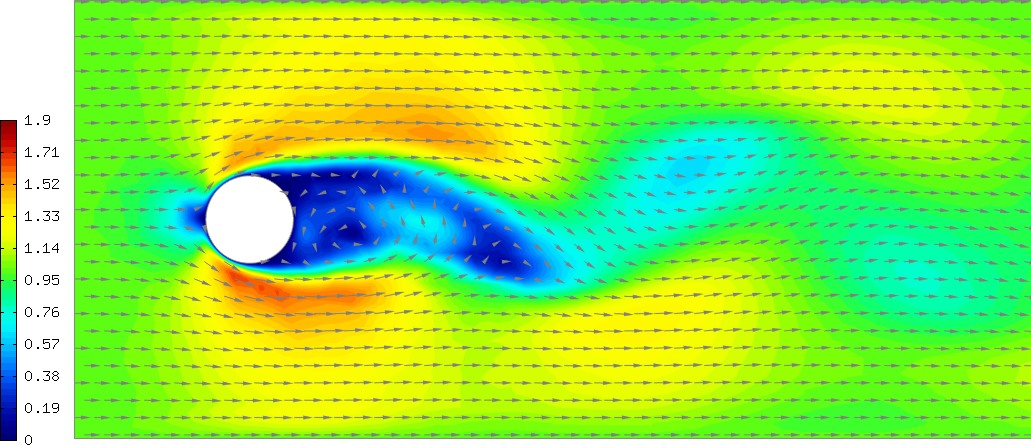
\includegraphics[width=0.99\textwidth]{img/velocity.jpg}
  \caption{Velocity solution visualized with {\tt VectorView}.}
  \label{fig:velocity}
\end{figure}


%%%%%%%%%%%%%%%%%%%%%%%%%%%%%%%%%%%%%%%%%%%%%%%%%%%%%%%%%%%%%%%%%%%%%%%%%%%%%%%%%%%%%%%%%%%%%%%%%%%%

\subsection{Automatic $hp$-adaptivity}

At this point you should be able to solve a large class of stationary and evolutionary PDEs
(or their systems) with Hermes2D. However, computations on a fixed mesh with fixed
polynomial degrees are not likely to be very accurate unless you uniformly refine the mesh
many times, which is expensive. There is a need for an {\it adaptive algorithm} designed
to improve the quality of the computation by refining the mesh and/or polynomial degrees
in areas of the domain where the approximate solution is too inaccurate.

Typically, one employs classical residual-based error estimation techniques to obtain an
error measure for each element. Elements with the largest error are then split ($h$-refined)
and the approximate solution is recalculated, which leads to an adaptive scheme known as
$h$-adaptivity. However, residual-based error estimation usually only works for elliptic
problems and lowest-order elements. Moreover, error convergence of the $h$-adaptive process
is only polynomial, which means it may be difficult to obtain very accurate solutions efficiently.

Another option is $p$-adaptivity, which increases polynomial degrees of elements with high
error indicator instead of splitting them. This is effective for smooth solutions, but in
general it is still insufficient. It turns out that in order to obtain very fast (exponential)
convergence, one must resort to $hp$-adaptivity, which allows simultaneous $h$- and $p$-refinements.
Figure \ref{fig:refinements} shows several examples of the many possible $hp$-refinements of
a fourth-order element.

\begin{figure}[ht]
  \medskip \centering
  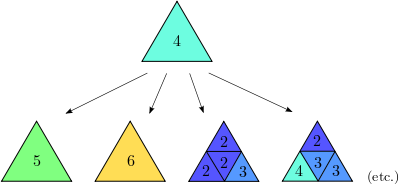
\includegraphics[width=0.9\textwidth]{img/refinements}
  \caption{Examples of $hp$-refinements.}
  \label{fig:refinements}
\end{figure}

However, due to the large number of options, classical error estimators in the form of one
number per element do not provide enough information to select the optimal $hp$-refinement.
One needs to know the {\it shape} of the approximation error in order to select the refinement
that leads to its maximum reduction. For this reason, $hp$-adaptive algorithms often employ
a~simple technique known as the {\it reference solution}. At each step of the adaptive process,
the current approximate solution is recalculated on a uniformly refined mesh and moreover
on elements with increased polynomial degrees. The reference solution is more accurate then
the standard coarse solution and subtracting the two gives an excellent and robust estimate
of the overall shape of the error.

The obvious disadvantage of the reference solution is its high computational cost (especially
in 3D). However, it is equation independent, works for elements of high order and can be
successfully used for $hp$-adaptivity, whose fast convergence compensates for the cost
of the reference solution.

Let us demostrate the use of automatic $hp$-adaptivity in Hermes2D on a simple problem of
electrostatics ({\tt examples/09-adapt}). The problem is concerned with the calculation of
the electrostatic potential in the vicinity of the electrodes of an electrostatic micromotor,
a miniature actuator device free of any coils. The problem is plane-symmetric.
Figure \ref{fig:micromotor} shows one half of the domain $\Omega$
(dimensions are given in millimeters).

\begin{figure}[ht]
  \medskip \centering
  \includegraphics[width=0.85\textwidth]{img/micromotor}
  \caption{Computational domain for the micromotor problem.}
  \label{fig:micromotor}
\end{figure}

The subdomain $\Omega_2$ represents the moving part of the domain and the area bounded by $\Gamma_2$
represents the electrodes that are fixed. Under some simplifying assumptions, the distribution
of the electrostatic potential $\varphi$ is governed by the equation
$$-\nabla\cdot\epsilon_r\nabla\varphi = 0,$$
equipped with the Dirichlet boundary conditions
$$\varphi = 0 V \ \ \ \ \ \mbox{on}\ \Gamma_1,$$
$$\varphi = 50 V \ \ \ \ \mbox{on}\ \Gamma_2.$$
The relative permittivity $\epsilon_r$ is piecewise-constant, $\epsilon_r = 1$ in $\Omega_1$ and
$\epsilon_r = 10$ in $\Omega_2$. The weak formulation reads
$$\int_\Omega \epsilon_r \nabla u \cdot \nabla v \dx = 0.$$
The varying parameter $\epsilon_r$ is handled by defining two bilinear forms in the code, one for
$\Omega_1$ and the other for $\Omega_2$. These two areas are delimited by element markers 1 and 2 in
the mesh, and the two forms are assigned to the corresponding markers during the registration of
the forms:
\begin{lstlisting}
 WeakForm wf(1);
 wf.add_biform(0, 0, biform1, SYM, 1);
 wf.add_biform(0, 0, biform2, SYM, 2);
\end{lstlisting}

The principal part of the example is the main adaptivity loop. In each iteration, the coarse problem
is solved first:
\begin{lstlisting}
 // solve the coarse problem
 LinSystem ls(&wf, &solver);
 ls.set_spaces(1, &space);
 ls.set_pss(1, &pss);
 ls.assemble();
 ls.solve(1, &sln);
\end{lstlisting}

Next, the reference solution must be obtained, which can be done by creating a refined copy of the mesh,
defining a temporary space with increased element orders and by assembling and solving an extra
linear system. However, for most problems, this can be automated using the class {\tt RefSystem}, which
handles all the temporary reference meshes and spaces transparently. All it needs is a pointer to our coarse
{\tt LinSystem}. The calculation of the reference solution is as simple as the following:
\begin{lstlisting}
 // solve the fine (reference) problem
 RefSystem rs(&ls);
 rs.assemble();
 rs.solve(1, &rsln);
\end{lstlisting}

In the third and last step of each iteration, we refine our mesh and polynomial degrees stored
in our space using a class called {\tt H1OrthoHP}. This class offers two services: it is able to
calculate  the estimate of the overall error of the coarse solution in $H^1$ norm, and if the
error is too large, you can ask the class to $hp$-adapt your mesh and element orders optimally.

{\tt H1OrthoHP} is initialized with the number of spaces in the problem and pointers to them.
The method \verb"calc_error" takes pointers to the coarse and reference solutions and returns
$$e = \frac{|| u - u_{ref} ||_{H^1}}{|| u_{ref} ||_{H^1}}.$$
You can test this value against a prescribed tolerance and exit the cycle if the tolerance is met:
\begin{lstlisting}
 H1OrthoHP hp(1, &space);
 if (hp.calc_error(&sln, &rsln) * 100 < tol) break;
\end{lstlisting}

Finally, we tell {\tt H1OrthoHP} to $hp$-refine all elements, whose error is larger than
0.3 times the largest error of all elements.
\begin{lstlisting}
 hp.adapt(0.3);
\end{lstlisting}

The computation starts with a very coarse mesh consisting of only 12 quadrilaterals, some
of which are moreover very ill-shaped. Thanks to the anisotropic refinement capabilities
of {\tt H1OrthoHP}, the mesh quickly adapts to the solution (Figure \ref{fig:motor-sln})
and elements of reasonable shape are created near singularities, which occur at the
corners of the electrode (Figure \ref{fig:motor-grad}). Initially, all elements of the
mesh are of degree one, but as the $hp$-adaptive process progresses, the elements receive
different polynomial degrees, depending on the local smoothness of the solution.
Usually, large elements of high degree are suitable for areas where the solution is smooth,
whereas tiny lowest-order elements are convenient near singularities
(Figure \ref{fig:motor-orders}).

The gradient in Figure \ref{fig:motor-grad} was visualized using {\tt VectorView}, which have
seen already in the previous section. Here, we plug in the same solution for both vector
components, but specify that its derivatives should be used:
\begin{lstlisting}
 gview.show(&sln, &sln, EPS_NORMAL, FN_DX_0, FN_DY_0);
\end{lstlisting}


\begin{figure}[ht]
  \medskip \centering
  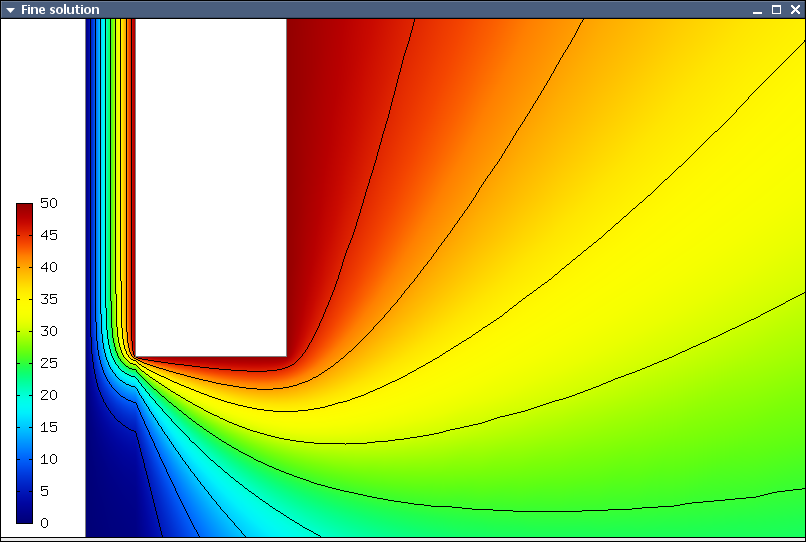
\includegraphics[width=0.95\textwidth]{img/motor-sln.png}
  \caption{Solution -- electrostatic potential $\varphi$ (zoomed).}
  \label{fig:motor-sln}
\end{figure}

\begin{figure}[ht]
  \medskip \centering
  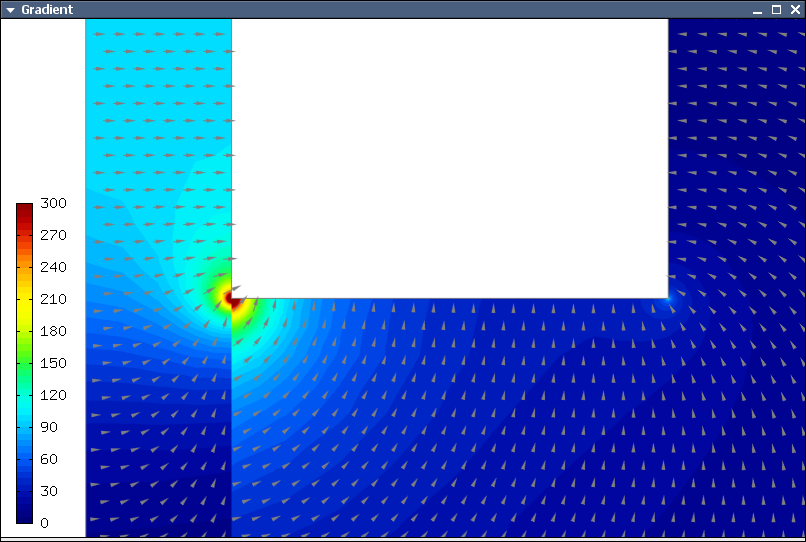
\includegraphics[width=0.95\textwidth]{img/motor-grad.png}
  \caption{Gradient of the solution $\bfE = \nabla\varphi$ and its magnitude (zoomed).}
  \label{fig:motor-grad}
\end{figure}

\begin{figure}[ht]
  \medskip \centering
  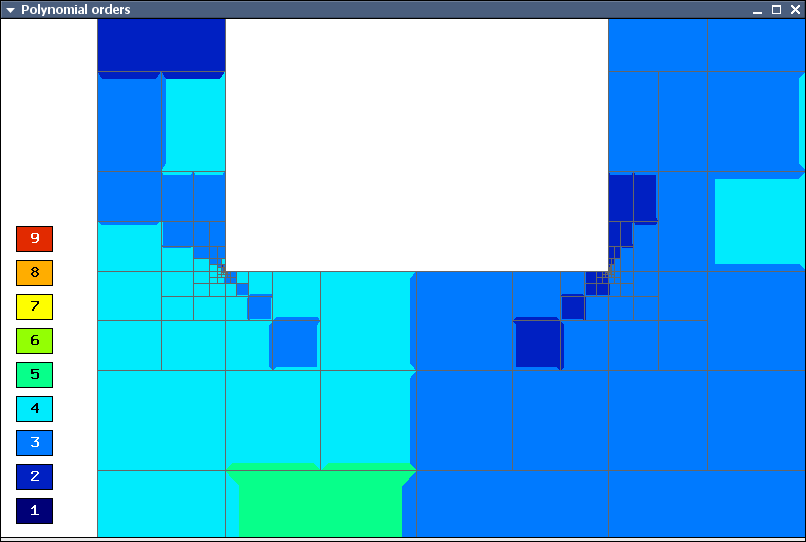
\includegraphics[width=0.95\textwidth]{img/motor-orders.png}
  \caption{Polynomial orders of elements near singularities (zoomed).}
  \label{fig:motor-orders}
\end{figure}

\clearpage

%%%%%%%%%%%%%%%%%%%%%%%%%%%%%%%%%%%%%%%%%%%%%%%%%%%%%%%%%%%%%%%%%%%%%%%%%%%%%%%%%%%%%%%%%%%%%%%%%%%%

\subsection{Adaptivity for Systems of PDEs}

It is possible to directly extend the procedure from the previous section to systems
of PDEs. For example, two spaces can be passed to {\tt H1OrthoHP}, four solutions (two coarse,
two reference) can be passed to \verb"calc_error_2" (see Section \ref{sec:h1adapt}) and finally
{\tt adapt} can be called as before. In this way, error estimates in $H^1$ norm are calculated
for elements in both spaces independently and the worst ones are selected and refined.

However, this approach fails for many systems, since their equations are usually coupled.
This means that the error in the solution of one equation can also affect other equations,
and it is not easy to recognize which elements should be refined to reduce the error.
Failure to refine the right elements may lead to stagnation in the convergence and even to a dead-lock.
In order to discover the sources of error, one has to know the structure of the coupling in the
system.

Recall that in elliptic problems the bilinear form $a(u,v)$ defines the energetic inner product,
$$(u,v)_e = a(u,v).$$
The norm induced by this product,
$$||u||_e = \sqrt{(u,u)_e},$$
is called the {\it energy norm}. \index{Energy norm} \index{Norm!energy}
It turns out that by measuring the error in the energy norm of the problem one can avoid the
above-mentioned difficulties. When calculating the error on an element, the energy norm accounts
also for the error caused by the element in other components of the solution, since it knows
all about the coupling of the equations. This is not the case for
the generic $H^1$ norm applied separately to the components.

Let us return to the equations of linear elasticity in Section \ref{sec:systems}. Our task
will be once again to determine the deformation of an elastic body subject to external forces.
Our domain (Figure \ref{fig:bracket}) is a model of a bracket loaded on its top edge and fixed
to a wall on the right edge, i.e.,
\begin{eqnarray*}
  \bfu \!&=&\! 0 \ \ \ \ \ \rm{on}\ \Gamma_1  \\
  \dd{u_2}{n} \!&=&\! f \ \ \ \ \ \rm{on}\ \Gamma_2 \\
  \dd{u_1}{n} = \dd{u_2}{n} \!&=&\! 0 \ \ \ \ \ \rm{elsewhere.}
\end{eqnarray*}
The dimensions are L = 0.7 m, T = 0.1 m and the force $f = 10^3$ N.

\begin{figure}[ht]
  \medskip \centering
  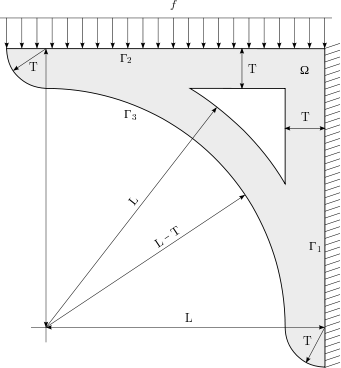
\includegraphics[width=0.65\textwidth]{img/bracket}
  \vspace{-2mm}
  \caption{Computational domain for the elastic bracket problem.}
  \label{fig:bracket}
\end{figure}

The implementation, located in {\tt examples/10-adapt-system}, is very similar to the micromotor
example from the previous section. Again, the coarse and reference solutions are calculated
in the main loop, only this time we have two equations in the system, two meshes, two spaces, etc.
The only substantial difference is in the calculation of the error estimate. Instead of
\verb"calc_error()" we use the method \verb"calc_energy_error()", also a member of the
class \verb"H1OrthoHP":

\begin{lstlisting}
 H1OrthoHP hp(2, &xdisp, &ydisp);
 error = hp.calc_energy_error_2(&xsln, &ysln, &xrsln, &yrsln,
                    bilinear_form_0_0, bilinear_form_0_1,
                    bilinear_form_1_0, bilinear_form_1_1) * 100;
\end{lstlisting}

The arguments of \verb"calc_energy_error()" are: $n$ coarse solutions, $n$ reference solutions,
and finally $n \times n$ pointers to bilinear forms of the problem (row after row), which are used
for the calculation of the energy norm of the error.

(The function \verb"calc_energy_error_2()" used above is a type-safe wrapper for the
more general function \verb"calc_energy_error()", which takes a variable number of arguments,
see Section \ref{sec:calc_energy_norm}).

\begin{figure}[p]
  \medskip \centering
  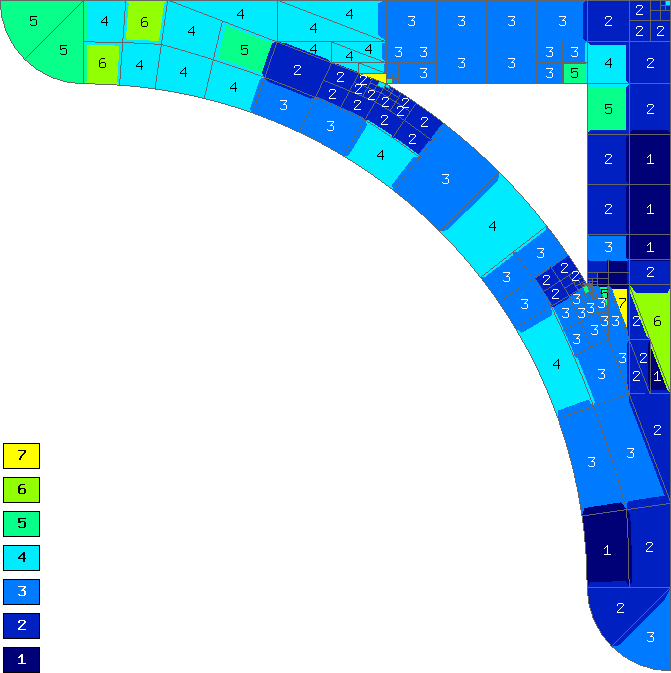
\includegraphics[height=0.43\textheight]{img/sys-xorders.png}
  \caption{$x$ displacement -- mesh and polynomial degrees.}
  \label{fig:sys-xorders}
\end{figure}

\begin{figure}[p]
  \medskip \centering
  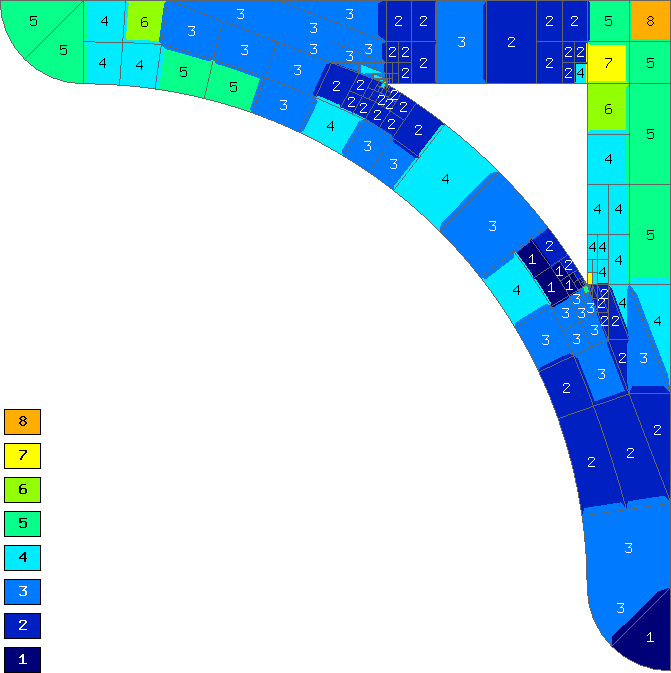
\includegraphics[height=0.43\textheight]{img/sys-yorders.png}
  \caption{$y$ displacement -- mesh and polynomial degrees.}
  \label{fig:sys-yorders}
\end{figure}

Figures \ref{fig:sys-xorders} and \ref{fig:sys-yorders} show the two meshes and their polynomial
degrees after several adaptive steps. Note that they are slightly different, not only in
polynomial degrees, but also in element refinements. This is possible in Hermes2D thanks to
a technique called multi-mesh assembling (see Section \ref{sec:multimesh}), which allows
all components of the solution to adapt independently. In problems whose components exhibit
substantially different behavior, one may even obtain completely different meshes.

\clearpage

%%%%%%%%%%%%%%%%%%%%%%%%%%%%%%%%%%%%%%%%%%%%%%%%%%%%%%%%%%%%%%%%%%%%%%%%%%%%%%%%%%%%%%%%%%%%%%%%%%%%

%\subsection{Summary}



%\begin{figure}[ht]
%  \medskip \centering
%  \includegraphics[width=0.7\textwidth]{img/collab}
%  \caption{Classes}
%  \label{classes}
%\end{figure}


\newpage
